%%%%%%%%%%%%%%%%%%%%%%%%%%%%%%%%%%%%%%%%%%%%%%%%%%%%%%%%%%%%%%%%%%%%%%
% LaTeX Example: Project Report
%
% Source: http://www.howtotex.com
%
% Feel free to distribute this example, but please keep the referral
% to howtotex.com
% Date: March 2011 
% 
%%%%%%%%%%%%%%%%%%%%%%%%%%%%%%%%%%%%%%%%%%%%%%%%%%%%%%%%%%%%%%%%%%%%%%
% How to use writeLaTeX: 
%
% You edit the source code here on the left, and the preview on the
% right shows you the result within a few seconds.
%
% Bookmark this page and share the URL with your co-authors. They can
% edit at the same time!
%
% You can upload figures, bibliographies, custom classes and
% styles using the files menu.
%
% If you're new to LaTeX, the wikibook is a great place to start:
% http://en.wikibooks.org/wiki/LaTeX
%
%%%%%%%%%%%%%%%%%%%%%%%%%%%%%%%%%%%%%%%%%%%%%%%%%%%%%%%%%%%%%%%%%%%%%%
% Edit the title below to update the display in My Documents
%\title{Project Report}
%
%%% Preamble
\documentclass[paper=a4, fontsize=10pt]{scrartcl}
\usepackage[T1]{fontenc}
\usepackage{fourier}
\usepackage{caption}
\usepackage[english]{babel}							% English language/hyphenation
\usepackage[protrusion=true,expansion=true]{microtype}	
\usepackage{amsmath,amsfonts,amsthm} % Math packages
\usepackage[pdftex]{graphicx}	
\usepackage{url}
\usepackage{wrapfig}
\usepackage{multirow}
\usepackage{hyperref}

\usepackage{sidecap}
%%% Custom sectioning
\usepackage{sectsty}
\allsectionsfont{\centering \normalfont\scshape}
%\PreviewEnvironment[{[]{}}]{tabular,enumerate}
\usepackage{geometry}
 \geometry{
 a4paper,
 total={210mm,297mm},
 left=10mm,
 right=10mm,
 top=10mm,
 bottom=10mm,
 }
%%% Custom headers/footers (fancyhdr package)
\usepackage{fancyhdr}
\pagestyle{fancyplain}
\fancyhead{}											% No page header
\fancyfoot[L]{}											% Empty 
\fancyfoot[C]{}											% Empty
\fancyfoot[R]{\thepage}									% Pagenumbering
\renewcommand{\headrulewidth}{0pt}			% Remove header underlines
\renewcommand{\footrulewidth}{0pt}				% Remove footer underlines
\setlength{\headheight}{13.6pt}


%%% Equation and float numbering
\numberwithin{equation}{section}		% Equationnumbering: section.eq#
\numberwithin{figure}{section}			% Figurenumbering: section.fig#
\numberwithin{table}{section}				% Tablenumbering: section.tab#


%%% Maketitle metadata
\newcommand{\horrule}[1]{\rule{\linewidth}{#1}} 	% Horizontal rule

\title{
		%\vspace{-1in} 	
		\usefont{OT1}{bch}{b}{n}
		\normalfont \normalsize \textsc{University Of Bristol / LaL Orsay} \\ [25pt]
		\horrule{0.5pt} \\[0.4cm]
		\huge Assessments \\
		\horrule{2pt} \\[0.5cm]
}
\author{
		\normalfont 								\normalsize
        Renato Quagliani\\[-3pt]		\normalsize
        \today
}
\date{}


%%% Begin document
\begin{document}
\maketitle
\section{Overview of work done}
A description of the work done during the first part of my PhD will be described in this document. It consists in two major blocks. The first one covers the physics analysis work and it has been performed between June 2014 and October 2014. At the same time i was completing the master degree in Ferrara Unviersity and as well as the NPAC master 2 at Paris Sud University. The second part of the document describes the work done in the context of the preparation for the upgrade of the LHCb detector. I worked on the improvement of a tracking as well as the development of a new algorithm: the \textit{Hybrid Seeding}.
%The analysis work regards the study of double charm $B$ decays at \textit{LHCb} while the \textit{Seeding Algorithm for the LHCb upgrade} connsists in a software development project.
%\subsection{Track Reconstruction project : Seeding Algorithm for the LHCb Upgrade}
Before getting to the heart of the work, an introduction about the tracking and the upgrade of the \textit{LHCb} detector is mandatory.
\subsection{Indtroduction to LHCb and to the Upgrade Scintillating Fibre Tracker (SciFi).}
The \textit{LHCb} detector ~\cite{Blake1} aims at search indirect signatures of New Physics through quantum loop induced processes through the measurements of strongly suppressed Standard Model processes.
In this context precision plays a fundamental role. 
Up to now, in \textit{LHCb} and other \textit{LHC} experiments, no strong deviations from the Standard Model (SM) have been observed and even if \textit{LHCb} has already provided the world's best measurements in many channels, it is still limited from improving them by statistics rather than systematics. Due to this, the upgrade of the \textit{LHCb} forward spectrometer is mandatory in order to collect \textit{O(100)} times more data and reduce the statistics uncertainty of a factor 10 in order to be comparable with the theoretical one ~\cite{Blake2}~\cite{Blake3}. On top of that the huge amount of collected data expected for the upgrade at $\sqrt{s} = 14$ TeV will be $\sim 5$fb$^{-1}$ per year  will also strongly improve our actual knowledges about \textit{QCD} and the dynamic of \textit{b} and \textit{c} hadrons decays, which is crucial for theoretical predictions and error estimations also on crucial analysis for the CP violation processes studied at \textit{LHCb}. The detailed description of the physics plan for the upgrade can be found in ~\cite{LetterIntent}

The \textit{LHCb} detector is a single-arm forward spectrometer aiming to detect particles and their decay products, and as the \textit{b} in the name of the detector suggests, it is designed to study particles containing \textit{b} and \textit{c} quarks which are produced strongly boosted in the forward direction for symmetric energies of colliding protons at $\sqrt{s}$=14 TeV.%\footnote{The relevant process infact is the quark-gluon fusion which can be obtained in proton proton collisions only with strongly asymmetric PDFs.}
The detailed description of the \textit{LHCb} detector can be found in ~\cite{Blake1}.
The data taking at \textit{LHCb} during 2011 ($\sqrt(s)=$7 TeV) and 2012 ($\sqrt(s)$=8 TeV) at \textit{LHCb} are mainly determined by few steps:
\begin{itemize}
\item{Interesting events are selected by the \textit{L0 Trigger} which is implemented at the hardware level aiming to reduce the 40 \textit{MHz} bunch crossing rate to 1\textit{MHz} making use of estimations and measurements of the signature of particles having high $E_{T},p_{T}$ through the muon stations and the calorimeters. The main reason why this is done is because the read-out system of some of the detector cannot afford an incoming rate of 40\textit{MHz}. In the upgrade, infact, all the read-out will be substituted and the \textit{L0} trigger will be replaced by a software one.}
\item{\textit{High Level Trigger (HLT) and Offline reconstruction}: the \textit{HLT} consists in an \textit{Online} software trigger where the full reconstruction of tracks is performed. It's at this level that the tracking algorithms are run. After the \textit{HLT}, data are stored and an \textit{Offline} reconstruction is also performed before providing usable object for data analysis. \footnote{During the Run-I, the seeding algorithm (called \textit{PatSeeding}) in the \textit{HLT} was run making use of the left-over hits coming from the \textit{Forward} algorithm. During Run-I the \textit{Seeding} was used in the online reconstruction in tandem with the \textit{Forward} as described before while in the offline reconstruction it was run as a \textit{Standalone} algorithm. For the Run-II online and offline reconstruction gives more or less the same results, but, anyway, the seeding algorithm remains one of the most important one.} Finally data are \textit{Stripped}, meaning that additional cuts are applied before their convertion in usable objects for data analysis.}
\item{\textit{LHCb} luminosity is kept constant and it's reduced with respect to other \textit{LHC} experiments of 2 orders of magnitudes. This reduction in luminosity is achieved thanks to the \textit{Luminosity Levelling} mechanism which avoid head-on collisions separating beams perpendicularly to the collision plane. This reduction of luminosity is mandatory since the main studies on \textit{b} and \textit{c} hadrons require an extraordinary precise reconstruction of the production vertices of the produced and dacaying particles, so, the VErtex LOcator (\textit{VELO}) can be placed at very small distance from the interaction point limiting problems coming from radiation damages. \footnote{The decrease from the maximal designed luminosity of \textit{LHC} of $10^{34}$cm$^{-2}s^{-1}$ to the \textit{LHCb} one  $10^{32}$cm$^{-2}s^{-1}$ permit to reduce the average number of inelastic collisions from 27 to 0.53 and it allows to reconstruct with extraordinary precision the primary vertices.}}
\end{itemize}

Regarding the upgrade, a brief description on what it consists is mandatory. A small summary is given in table ~\ref{table:runningCondition} where $\nu$ stands for the average number of visible interaction per bunch crossing.

\begin{table}[h]
\centering
\begin{tabular}{|c|c|c|}
\hline
           & \textbf{Current \textit{LHCb}}          & \textbf{Upgrade \textit{LHCb}} \\ \hline
Trigger    & Hardware(\textit{L0}) + Software(\textit{HLT}) & Only Software \\ \hline
Read-out rate & \textit{L0}: 40 \textit{MHz} to 1\textit{MHz} for readout & 40 \textit{MHz} Full software trigger for every 25 ns bunch crossing \\ \hline
Luminosity & $4 \times 10 ^{32}$cm$^{-2}s^{-1}$ & $2\times 10^{33}$cm$^{-2}s^{-1}$ \\ \hline
$\nu $ & 2 & 7.6 \\ \hline

\end{tabular}
\caption{Main differences between actual LHCb and the Upgrade}\label{table:runningCondition}
\end{table}

The reason why the \textit{L0} trigger will be removed in the upgrade is mainly because lot of analysis looking for deviations from Standard Model at \textit{LHCb} are limited by statistics and a fixed 1 \textit{MHz} readout at the upgrade running condition will be too limiting. 
In order to reach the physics goals the \textit{LHCb} detector will be upgraded and the installation of the new detectors and the new read-out is expected to happen during the long shutdown 2 in 2018/2019.
Each subdetectors will be replaced as shown in Fig.~\ref{Fig:Upgrade}.
\begin{figure}[h]
  \begin{center}
    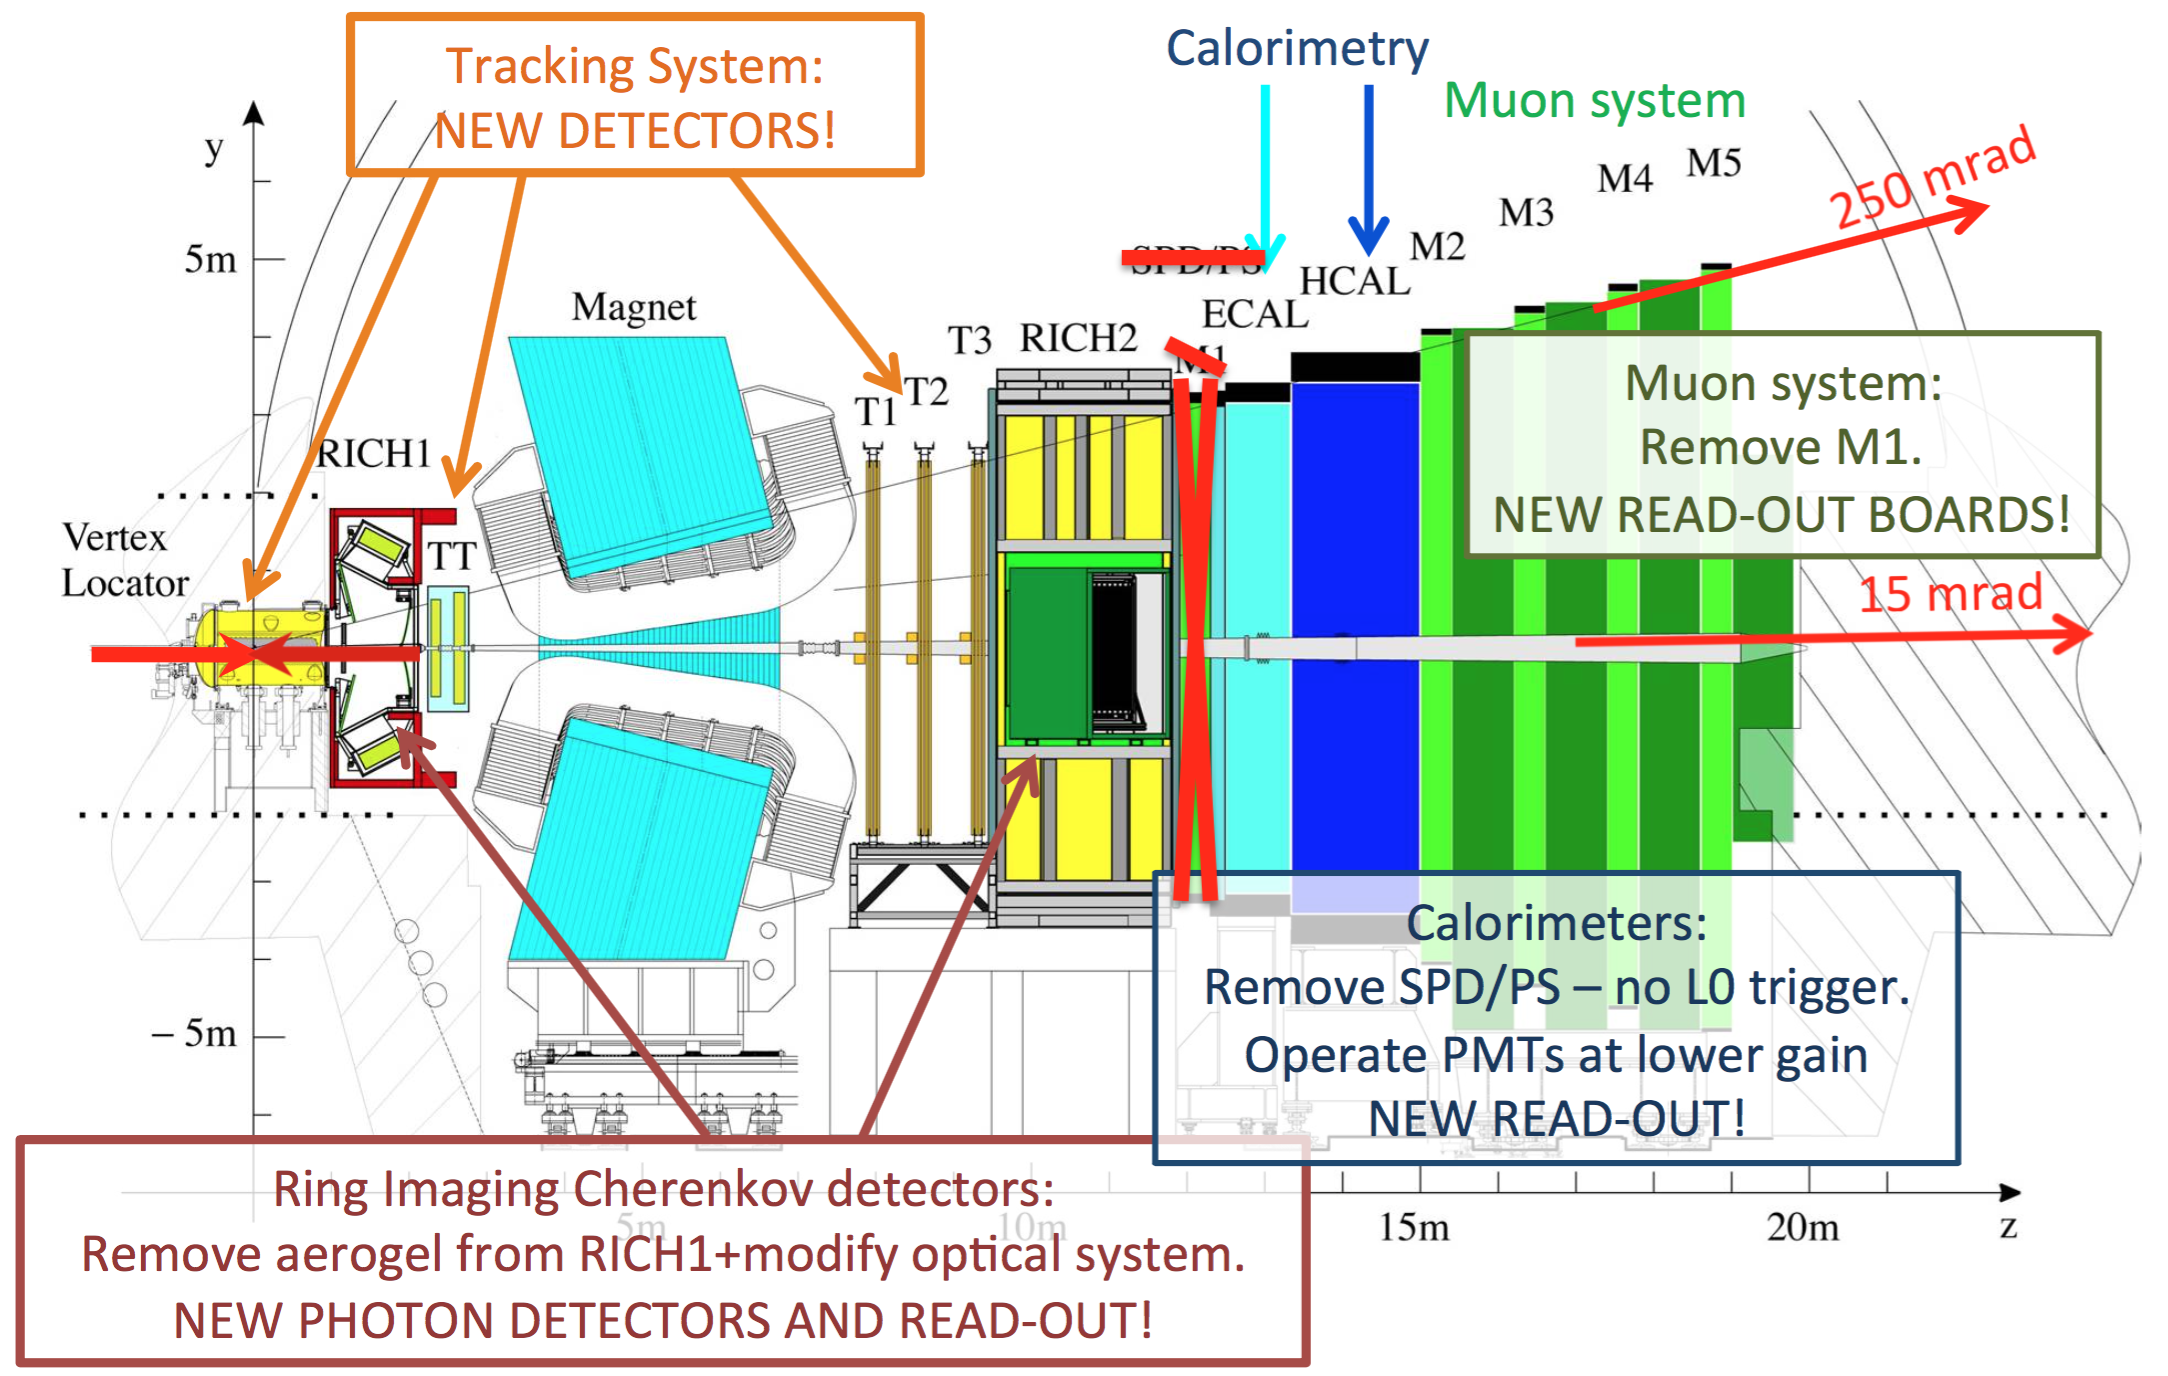
\includegraphics[width=0.5\textwidth]{Images/Upgrade.png} 
  \caption[Caption for track type]{LHCb detector modifications for the upgrade. The Vertex Locator (\textit{VELO}), the Tracker Turicensis(\textit{TT}) and the 3 T-Stations are the main resposible of the tracking at LHCb. The Particle Identification is ensured by the two ring cherenkove detectors (\textit{RICH1} and \textit{RICH2}). The particles energy measurement is provided by the hadronic and the electromagnetic calorimeters (HCAL and ECAL respectively). The properties of the muons are then mainly determined by the Muon System.}\label{Fig:Upgrade}
  \end{center}
\end{figure}

The actual \textit{VELO} will be replaced by a lightweight hybrid pixel detector capable of 40 $MHz$ readout at the upgrade luminosity which is 5 times greater than the actual one.
%Regarding the \textit{PID} detectors (\textit{RICH1 and RICH2}), the aerogel from \textit{RICH1} will be removed and the opitcal system will be modified, and , of course , new photon detectors and read-out system will be implemented. Since the \textit{L0} trigger will not be present in the upgrade, so the Scintillating Pad detector and the pre-shower which basically initiate the electromagentic and hadronic shower and applies some vetoes to the events will be removed. The calorimeters will remain the same apart of the implementation of a new read-out. The muon system also will remain the same apart of a new read out and the removal of the first station (\textit{M1}).
The trackers placed downstream and upstream with respect to the magnet will be also completely replaced. In particular, the downstream tracker which is actually made by the so-called Inner tracker (\textit{IT}) and the Outer Tracker (\textit{OT}) will be replaced by the scintillating fibre tracker (\textit{SciFi}) detector to cope for the higher luminosity, higher occupancy and the 40 \textit{MHz} read-out.

The current tracker system downstream the magnet implement two different technologies: the \textit{OT} system is based on gaseous straw tube detector for a global resolution on the bending plane (\textit{x-z}) of around 200 $\mu m$ while the Inner Tracker is made of Silicon microstrip detectors ( also employed for the \textit{Upstream Tracker} upgrade).
%The main reason why it's necessary to replace the \textit{IT} and \textit{OT} is related to the occupancy being too high in upgrade conditions and the fact that the electronics for them was designed for a 1MHz read-out rate. 
Anothe reason why it's necessary to replace them is related to the fact that for the upgrade phase of \textit{LHCb} an integrated luminosity greater than 50 fb$^{-1}$ is expected to be collected and the detector itself is required to be resistent to the corresponding radiation damages.

The adopted solution for the downstream magnet upgrade is the \textit{Scintillating Fibre Tracker} (\textit{SciFi}). The active and light-transport (also wavelenght shifter) material for the detector are the fibres themselves and the read-out is provided by arrays of silicon photomultipliers. The pitch of a single channel is designed to be equal to 250 $\mu m$ and each module of the detector consist of 5 (6 in central region) closed packed fibres ($\Phi \sim 250 \mu m$) layer.

 
The \textit{SciFi} is placed in the downstream region with respect to the magnet (\textit{B} field lines direction are along the \textit{y} direction) and it consists of 3 stations, \textit{T1,T2,T3} being \textit{T1}($z\sim 8m$) the station closer to the magnet and \textit{T3} ($z\sim 10m$) the one closer to the calorimeter. Each station is composed by four layers of scintillating fibres detectors oriented in the so-called \textit{x-u-v-x} configuration.\footnote{The x - layer contains fibres oriented perpendicularly to the x-z plane while the u(v) layers are exactly the same as the x-layers but rotated by a ``stereo'' angle of +5(-5) degree in the x-y plane in order to reconstruct also the y-information of the tracks.}

This configuration (\textit{x-u-v-x}) allows the reconstruction of tracks using their projection in the bending \textit{x-z} plane and the evaluation of the \textit{y} information is obtained through the combined measurement of the \textit{u-v} layers. 

Each layer is divided in two halves (roughly \textit{y>0} and \textit{y<0}) equipped at \textit{y=0} by a mirror to improve the light yield in the higher occupancy area (the region close to the beam pipe).

A skematic view of how a single station look like is given in ~\ref{Fig:SciFi} and it will consists of around 10.000 \textit{Km} of fibres and 560.000 read-out channels distributed over the 12 layers (6 \textit{x}, 3\textit{u}, 3\textit{v}).
\begin{figure}[h]
  \begin{center}
    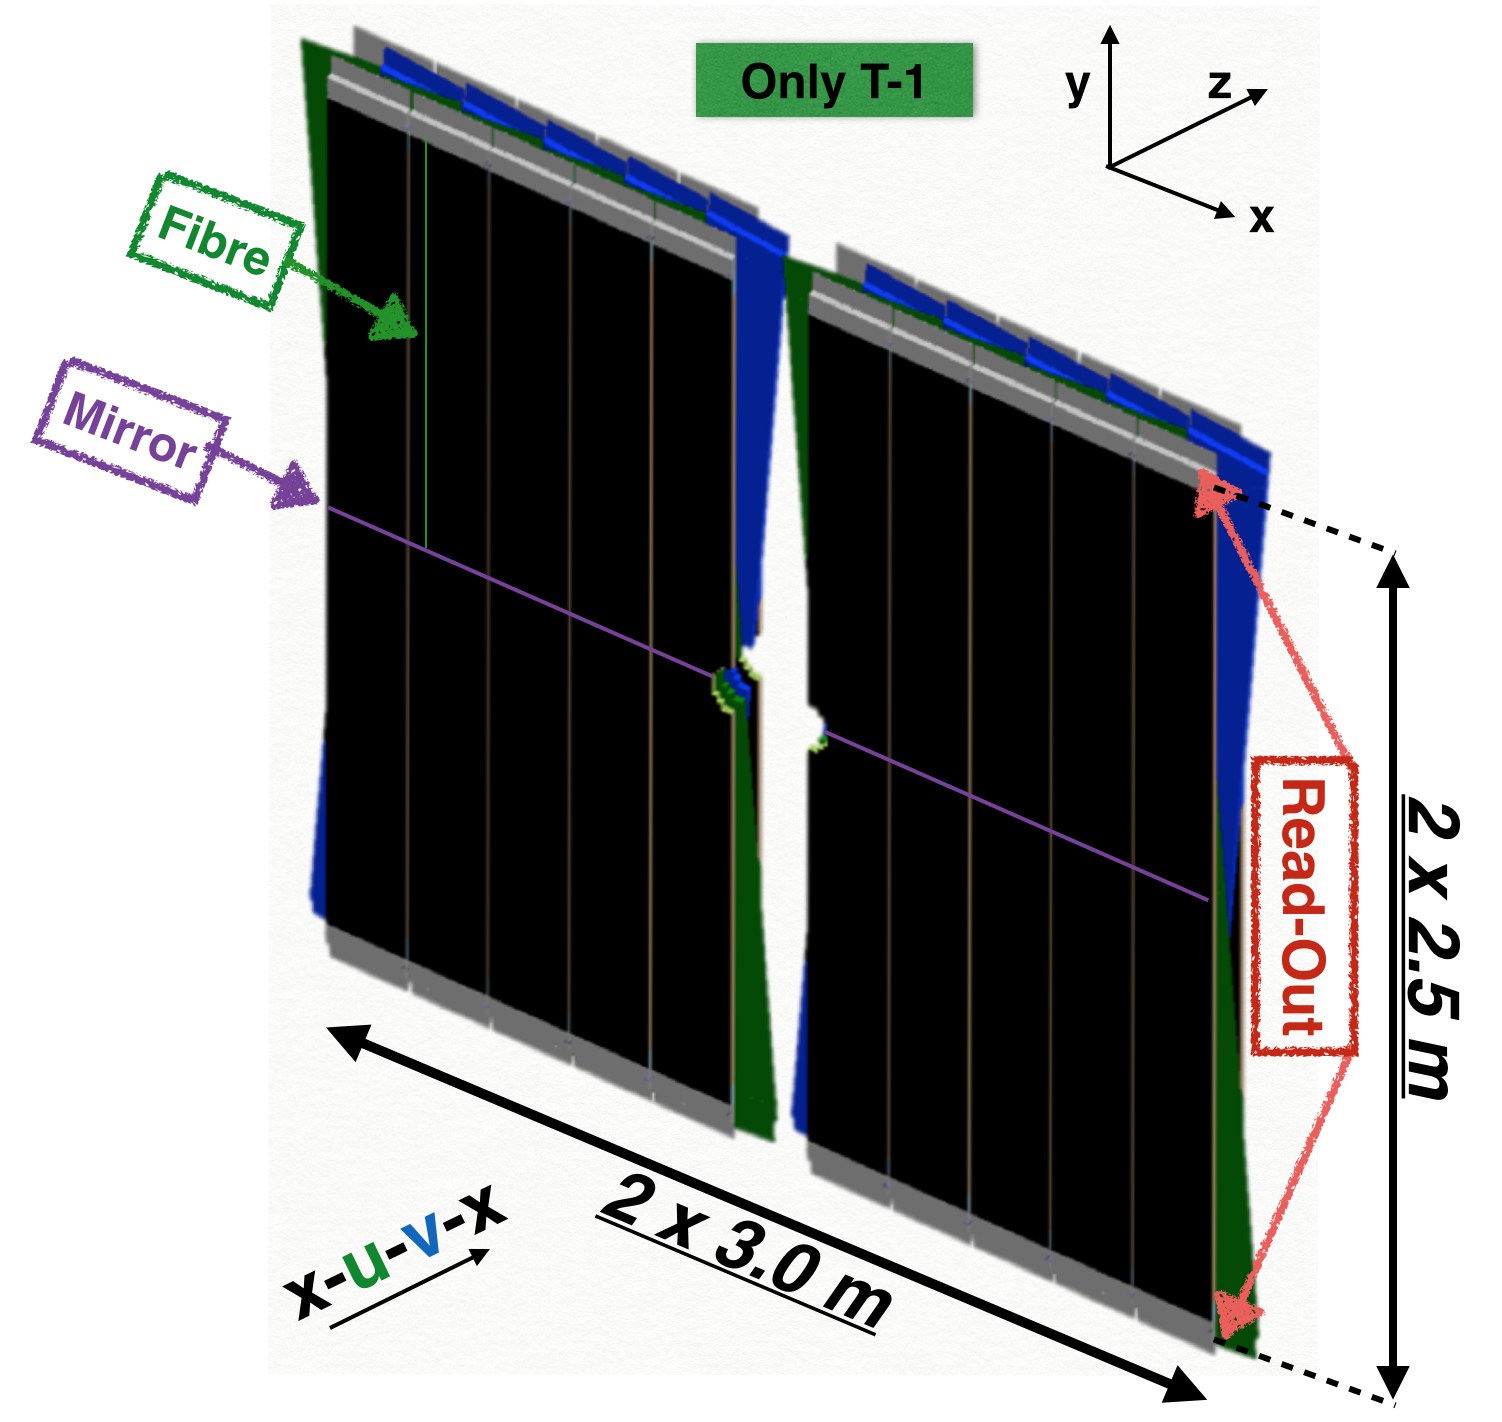
\includegraphics[width=0.5\textwidth]{Images/ModuleSciFi.png} 
  \caption[Caption for track type]{\emph{Sketch of a single station of the SciFi tracker. Each station is made of 4 different layers in x-u-v-x configuration, the central region is mirrored and the read-out is done at the edges of the layers far from the beampipe.}}\label{Fig:SciFi}
  \end{center}
\end{figure}

The requirements for the \textit{SciFi} to satisfy the physics program of \textit{LHCb} can be listed in few concise points: 
\begin{itemize} 
\item{The hit efficiency has to be $\sim 99 \%$.}
\item{The noise cluster rate should be less than 10$\%$, reason why the \textit{SiPM} read-out has to be cooled}\item{The position resolution in the bending plane has to be $\sim 100 \mu m$ and the material budged has to be as reduced as possible $\frac{X}{X_{0}}<1 \%$ per detector layer.}
\item{The read-out has to be performed at 40 \textit{MHz}.}
\item{The tracker has to be efficient for at least an integrated luminosity of 50 fb$^{-1}$.}
\item{The \textit{SciFi} tracker has to replace the actual one, so additional goemetrical constraints must be satisfied.}
\end{itemize}

\subsection{Pattern recognition at LHCb}

%Regarding the track reconstruction in the standalone seeding algorithm the most important thing is the geometrical arrangements of the module which is the same as the current detector due to geometrical contraints. A detailed description of the \textit{SciFi} tracker can be found in ~\cite{TDR_SciFi}. 

%%%Track Reconstruction
The track reconstruction at \textit{LHCb} is performed in different steps. The idea is to first reconstruct tracks collecting a list of hits from sub-detectors following some given criteria. For example the track model itself can be a criteria to look for compatible hits given a subdetector since the expected behavior of tracks in between one detector and another change due to the shape of the \textit{B} field in a given sub detector.

All the found tracks are stored in a temporary container and a global fit and finer treatment is performed afterwards (\textit{Kalman Filter} and also a \textit{Ghost and Clone killer} procedure is applied. We will then refer to the first step as \textit{pattern recognition} and the second one as the \textit{final fit}. 

The pattern recognition at \textit{LHCb} is done depending on the path the track goes through, so it's based on the datector's hit content as shown in Fig. ~\ref{figure:Tracks}.
\begin{figure}[h]
  \begin{center}
    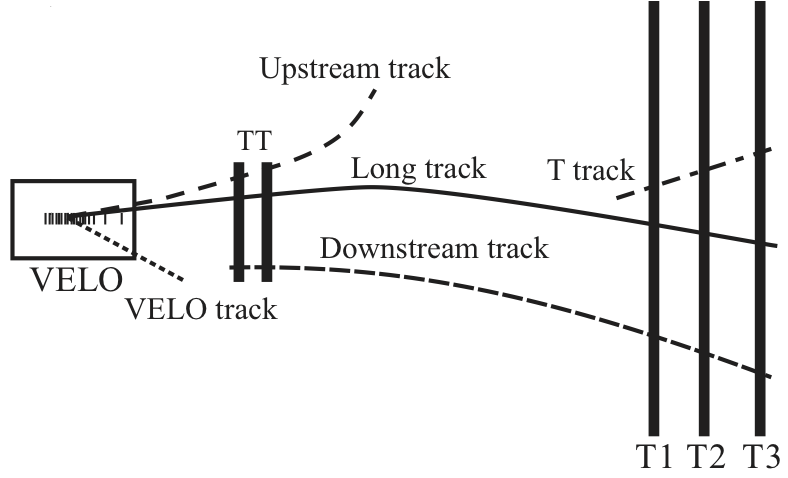
\includegraphics[width=0.5\textwidth]{Images/tracktype.png} 
  \caption[Caption for track type]{\emph{Track type at \textit{LHCb}. Velo tracks are basically straight lines since the magnetic field is almost 0 in that region. Tracks are mainly bended in the x-z \footnotemark plane between the Tracker Turicensis (Upstream Tracker for the upgrade) and the T-Stations which is composed by the Inner Tracker(IT) and the Outer Tracker(OT) (Run-I and Run-II), while for the upgrade the stations will be replaced by the Scintillating Fibre tracker (SCIFI).}}
  \label{figure:Tracks}
  \end{center}
\end{figure}

\footnotetext{ z- is the beam axis direction and the y axis is the B field line direction.}
In the tracking system of \textit{LHCb} each track type is reconstructed by a dedicated algorithm and a schematic layout of how it is done is given in table \ref{Table:tracks}.
\begin{table}[h]
\begin{tabular}{|l|l|l|l|l|}
\hline
Track type & Used detector &Algorithm(s)& Input tracks&  Output tracks    \\ \hline
\begin{tabular}[|l|]{@{}l@{}}Velo Tracks\\ or Velo-Segment\end{tabular} & Velo & Velo algorithm  & \multicolumn{1}{|l|}{/} & Velo         \\ \hline
\begin{tabular}[|l|]{@{}l@{}}Seed Tracks\\ or T-Tracks\end{tabular}     & \begin{tabular}[|l|]{@{}c@{}}T-Stations\\ (SciFi in upgrade)\end{tabular}                                                                                    & \multicolumn{1}{|l|}{Seeding algorithm}                                                                                             & \multicolumn{1}{|l|}{\begin{tabular}[|l|]{@{}l@{}}Allow the possible \\usage of the \\leftover hits of forward.\\ If Not: Standalone Algo\end{tabular}} & Seed  \\ \hline
\multicolumn{1}{|l|}{\multirow{2}{*}{Long Tracks (1)}}                  & \multirow{2}{*}{\begin{tabular}[l]{@{}l@{}}Velo + TT + T-Stations\\ (TT $\rightarrow$ UT  \\ T-Stations $\rightarrow$ SciFi \\ in upgrade)\end{tabular}} & \begin{tabular}[|l|]{@{}l@{}} 1) Forward tracking:\\ Search in T-Stations knowing \\ Velo-Segment (adding also TT)\end{tabular}         & Velo               & \multirow{2}{*}{Long} \\ 
\multicolumn{1}{|l|}{}                                              &                                                                                                                                                            & \begin{tabular}[|l|]{@{}l@{}} 2)Matching algorithm:\\ Merge T-Tracks with Velo-Segment\\ 3)BestSelector= Forward+Matching\end{tabular} & Velo and Seed& \\ \hline
Downstream Tracks & \multicolumn{1}{|l|}{\begin{tabular}[|l|]{@{}l@{}}T-Stations and TT\\ (SciFi and UT)\end{tabular}}& \begin{tabular}[|l|]{@{}l@{}}Downstream algorithm:\\ Use T-Tracks and\\ add TT (UT upgrade) hits\end{tabular}& Seed& Downstream            \\ \hline Upstream Track & \multicolumn{1}{|l|}{Velo and TT} & \begin{tabular}[|l|]{@{}l@{}}Upstream algorithm:\\ Use Velo segment and \\ add TT( UT upgrade) hits\end{tabular} & Velo Container &  Upstream \\ \hline \end{tabular}
\caption{\emph{Pattern recognition at LHCb}}\label{Table:tracks}

\end{table}

All the tracks produced by the algorithms provided in table ~\ref{Table:tracks} are processed afterwards by the \textit{Kalman Filter} which fit the tracks assigning a \textit{univoque} $\chi^{2}$ value to the tracks. Infact, each algorithm has an internal track model parametrisation and the global effect comparing different algorithms is to have different $\chi^{2}$ value for the same track, for instance and in addition pattern recognition algorithm are not expected to correct the fit for multiscattering effects, it's infact the \textit{Kalman Filter} the algorithm where the fit takes into account the full \textit{B(x,y,z)} field map and the material budget computing at the same time the corrections due to multiscattering.

From a more technical point of view, in the \textit{Kalman Filter} and in the \textit{LHCb} framework each track is defined by a vector of track state $\left( x, y, t_{x}, t_{y} , \frac{q}{p} \right)_{z}^{T}$ where $t_x = \frac{dx}{dz}$ is the slope of the track in the \textit{x-z} plane at a given \textit{z},$t_y=\frac{dy}{dz}$ is the slope of the track in the \textit{y-z} plane at a given \textit{z}. In the \textit{Kalman Filter} the track state is propagated by a $5$x$5$ matrix through the detector considering the interactions in the material and the magnetic fiel map \footnote{The formalism is quite similar to accelerator physics for beam transport.}. 

The main goal of the pattern recognition algorithm in Table ~\ref{Table:tracks} is to provide a preliminary set of tracks made by compatible hits in a given sub-detector. Only at the end of the algotithms the found tracks (or, better, set of hits) are converted into a vector of track states, which can be handled by the \textit{Kalman Filter} and the \textit{Ghost and Clone Killer}.

\subsection{Hybrid Seeding Algorithm}
In order to figure out the limitations, exploit the future performances and eventually improve the baseline detector layout of the \textit{SciFi} tracker, a huge effort must be done to reproduce what the real data taking conditions togheter with  the real output of the detector would be. 

This task is obtained through different steps in the \textit{LHCb} simulation software. 
Without going into details we can make a short summary of how the \textit{LHCb} software is working in order to provide, for a given algorithm the final efficiencies. In this document reconstruction efficiencies are estimated for a simulated sample of  $B_s\rightarrow \phi\left( K^{+}K^{-}\right) \phi \left( K^{+}K^{-} \right)$ event.
\begin{itemize}
  \item{\textit{Gauss}: this application is responsible of the physics simulation, starting from the $pp$ collisions (package doing that is called \textit{Pythia8}). For the upgrade the 25 \textit{ns} bunch crossing, $\sqrt{s}= 14$ \textit{TeV} centre-of mass energy collision and the $\nu$\textit{=7.6} are passed as argument. After the collision simulation the subsequent $B_s\rightarrow \phi\left( K^{+}K^{-}\right) \phi \left(K^{+} K^{-} \right)$ decay is simulated (package \textit{EvtGen}).
 Inside \textit{Gauss} also the interaction in material of the produced final states in the detector is simulated by the \textit{Geant} package. At this level of the simulation the so-called \texttt{MCHits} are produced, corresponding to the energy deposition in the active material of the detector. A true particle is then given by a certain set of \texttt{MCHits}.}
%\item{Interactions in the material and geometrical acceptance effects are simulated inside the \textit{Gauss} package (interactions are done by \textit{Geant} software). The output of this step is the so-called \textit{MCHit}, and collections of \textit{MCHits} provides the so-called \textit{MCParticles}}.
\item{\textit{Boole}: this application is responsible of the read-out, the \textit{SiPm} response , the light attenuation in the fibres and the \textit{clusterization} together with the front-end boards ( data - encoding ) simulation. The output of this step are the \texttt{Clusters} containing binary information about the corresponding position in the tracker and additional information of the cluster such as the \textit{charge} and the \textit{cluster size}.}
\item{\textit{Brunel}: once the digitization is done, the resulting objects that the pattern recognition algorithms can handle are the so called \texttt{PrHit} (in the \textit{SciFi} context) and making use of them one can finally reconstruct tracks. The \texttt{PrHit} are obtained converting the binary information of the \texttt{Clusters} into a geometrical information usable for pattern recognition. The track reconstruction is done inside the \texttt{Brunel} application. It's clear that, if something goes wrong in the digitization or in the detector gemetrical information description, the pattern recognition algorithm will fail in the reconstruction, resulting in loss of tracking efficiencies.}
\item{\textit{Brunel checkers}: in order to provide the tracing reconstruction efficiencies, it is important to propagate the information of what we suppose to reconstruct if the pattern recognition algorithm would be 100$\%$ efficient. To do that, we store the \texttt{Linkers} inside \textit{Boole} in order to figure out the list of \texttt{MCHit} associated to the same true particle ending up into a \texttt{Cluster} ,i.e.,  into a \texttt{PrHit}. Thanks to these \texttt{Linkers} one can define the \textit{reconstructible}\footnote{For the \textit{SciFi} a reconstructible track is defined if it leaves at least 1 x-layer hit in each of the three stations together with at least one hit in the u or v layer for each of the three stations.} tracks and comparing them to the output of the pattern recognition algorithm (\textit{reconstructed} tracks) we are able to provide the pattern recognition efficiencies.}
\end{itemize}

The most important figures of merit used to evaluate the performances of a pattern recognition algorithm are the following:
\begin{itemize}
 \item{\textit{Reconstruction efficiency} : The track finding efficiency is defined as the fraction of \texttt{MC} particles in the acceptance that are successfully reconstructed,i.e, the percentage of \textit{reconstructed} tracks which are \texttt{MC-matched} (sharing the \textit{70} $\%$ of hit) among the set of \texttt{MCParticles} ending in the \textit{LHCb} acceptance. $$\epsilon = \frac{N_{MC-matched}}{N_{MC-acceptance}}$$.The acceptance is defined as at least one \textit{x} and one \textit{u} or \textit{v} layer hit per station.}
 \item{\textit{Ghost rate} : It is defined as the fraction of ghost tracks among the set of \textit{reconstructed} ,i.e., as the fraction of \textit{reconstructed} tracks not matched to a \texttt{MCParticle}.$$ghost_{rate} = \frac{N_{ghost}}{N_{reconstructed}}$$. Ghosts are generated from psudo-random combination of hits. This parameter is important because we don't want to recontruct fake tracks or use them in analysis, and, in addition, we don't want to feed the \textit{Kalman Filter} with too many fake tracks due to timing constraints.}
 \item{\textit{Timing} : It is defined as the time we spend to find the tracks in the algorithm. This is particualry important for the upgrade since the pattern recognition algorithms will run online at an incoming rate of \textit{40 MHz}.}
\end{itemize}

The work done from October 2014 to now is encoded in this framework. 

At the beginning i was involved in the debugging of the simulation code (\textit{Boole} and \textit{Brunel}), putting my hands in the detector description, the clusterisation and the encoding and decoding of the clusters to figure out the presence of some inconsistencies or wrong assumptions.

Some problems and inefficiencies in the software were infact not well understood passing from the default detector description (the one of the technical design report ~\cite{SciFiTDR}) to the new one where bigger gaps between channels were simulated, together with a new shape of detector layers, and a more realistic model of the clusterisation were implemented. 

In that context my effort was crucial (i took part to the ``\textit{DILBERT}'' task force for the software fixing and bug correction) to recover part of the loss in efficiency and we finally provide a stable version of the simulation of the detector from which the development of a new pattern recognition algorithm becomes possible. The discrepancies with the \textit{TDR} values were understood and the explaination to them are mainly related to the increased dead region due to the gaps in between two different readout channels.

In the meanwhile i partecipated to the \textit{Test Beam} data taking and data analysis aiming to measure the radiation lenght of the fibres doing light yield measurements scanning along the active material at different distances from the read-out and also evaluating the dependency of the cluster size against track incident angles. I also analyse some of the data from the test beam to study the cluster size properties as a function of the incident angle of tracks in the detector in order to tune the simulation to be the most reliable and realistic possible. ~\cite{AnalysisOrsay}.

The results of how the efficiencies for the seeding algorithm evolved since i started will be shown at the end of this section to highlight my contribution to the upgrade \textit{SciFi simulation and reconstruction} working group. I presented regularly my work in the internal \textit{SciFi simulation and reconstruction} working group and i presented once the results of the group in the parallel session of the \textit{LHCb week}. 

\subsection{Improvements apported to the algorithm}
Several trials in improving the previous algorithm (referred to \textit{Old} here) has been done. Once we figured out the limitations of it we decided to develop a new one from scratch. The developing of the new one started from very basics things related to track properties, detector occupancy and requirements on tracks.
First of all we need to separate different aspects of the algorithm: 

\begin{itemize}
\item{The way we collect the hits to generate tracks.}
\item{The way we fit the tracks.}
\item{The tolerances we allow in both the fitting and the hit search.}
\item{The requirements we put on tracks for their storage and clone/ghost killing.}
\end{itemize}

In order to do that, several tools have been developed: one of them, for instance, aims to extract the true \textit{Monte-Carlo} information of tracks before the clusterisation step in order to evaluate the track properties and their behavior in the \textit{SciFi} stations.\footnote{Thanks to that a tracking algorithm running over true hit position was developped to figure out which is the best track model to use in order to fit the tracks going through the \textit{SciFi} and also to have an estimation of ``how much'' one can squeeze some search windows without starting to loose too much in efficiencies.} The strategy adopted once the track property was extracted was then the following: instead of using a look-up table for the \textit{B} field information one can directly use the \textit{B}-field effect on tracks parametrising their motion by some fixed constants reflecting the magnetic field behavior.\footnote{The B field in the Sci-Fi tracker region is a fringe field which is not easly parametrisable, but still, some caractheristic behavior can be extracted.}

The main limitations, or problems, of the previous algorithm can be summarized in few points:
\begin{itemize} 
\item{It was trying to find everything at once, meaning that it was not disentangling the cases where tracks are easy to finde to the cases where the tracks are harder to find. Harder to find stands for find it paying an high prize in terms of ghost rate.}
\item{The tracks behavior in the \textit{SciFi} tracker was roughtly parametrised.} 
\item{The different detector area were treated in the same way even if where we expect a lower efficiency we can loosen the cuts for the track selection.}
\end{itemize}

The strategy adopted for the track search is to \textbf{split the algorithm in nested sub blocks} following the philosophy of the \textit{projective tracking} and \textit{progressive cleaning} of the tracking environment. Since the detector is divided into two halves (\textit{y>0}mm and \textit{y<0}mm) a natural choice is to split the algorithm in a first step where tracks are searched using only the hits in the upper modules of the stations and a second iteration is done using hits from the lower half. 
From the \textit{MC} study we find out that the amount of tracks going from the upper to the lower half is a negligible fraction of the full set of tracks \textit{$\sim O(0.1 \%)$}. 

Inside the upper(or lower) half search we run the second main block of the algorithm three times (we will call them \textit{cases}). For each \textit{case} different configurations for search windows and tolerances are applied. Each one of the \textit{case} is dependent on the previous one since at the end of each of them (only the first and the second) we mark the hits on the found tracks using some specific criteria. The net result is a progressive cleaning of the tracking environment moving from one case to the following one. For example in the second \textit{case} the hits found by the first one are not available for track reconstruction.
Each of the case is made by some different step:
\begin{itemize}
  \item{\textbf{\textit{x-Hit search}}: Hits are collected using only the \textit{x} layers in the 3 stations, so the maximal number of hits on track is 6 and the minimal one can be set to 4 or 5 depending on the case. The lower is the minimal number of hit required here the higher is the ghost rate since, for instance, tracks with only 4 x-layer hits are much less constrained than tracks with 6 x-layer hits.}
    \begin{enumerate}
    \item{2-Hit combinations are obtained looking at pairs of hits in the \textit{x-layers} in \textit{T1} and \textit{T3}. Given a hit in the first station (\textit{T1}) the infinite momentum prediciton is used to open a search window in \textit{T3} ($x_{T3} \sim \frac{x_{T1}}{z_{T1}}\cdot z_{T3}$ under the $p^{ \infty }$ assumption). All possible 2-hit combination are then collected. Tighter search window is applied for the first \textit{case} and bigger ones are used for the second and third one in order to find lower momentum tracks.}
      \item{All possible third hit from \textit{T2} is added to each single pair taking the linear predicition from $x_{T2} = \frac{x_{T3}-x_{T1}}{z_{T3}-z_{T1}}\cdot z_{T2}$. At this step, the small is the momentum of the track we are searching for and the bigger the deviation from the linear predicted position we should look for. This search window is correlated to the $p_{x}$ and to the sagitta of the track itself in the bending plane.}
      \item{Starting from 3 hit combination (one per station), the parameters of a parabola can be computed solving for $a_{x},b_x,c_x$ form the linear system given by $x_{i}(z_{T-i})= a_{x}+b_{x}\cdot dz_{T-i}+c_{x}dz_{T-i}^{2}$ where $dz_{T-i} = z_{T-i}-z_{ref}$ and $z_{ref}$ is picked to be $8530 mm$ ($\sim z_{T2}$) for numerical stability of track parameters ($a_{x},b_{x},c_{x}$).\footnote{In reality we solve for $(a_{x},b_{x},c_{x})$ using $x(z)=a_{x}+b_{x}dz+c_{x}dz^{2}(1+dRatio\cdot dz)$ where the \textit{dRatio} is fixed by MC studies}}
      \item{Once we have the $a_{x}$,$b_{x}$ and $c_{x}$ we can compute the predicted $x$ position at any $z$ and collect the found hits around the expected position inside a given tolerance. At this step the hit at the smallest distance from the prediction is picked and added to the track.}
      \item{At this stage, a list of hits is collected which should correspond to the \textit{x-z} projection of the true track in \textit{x-layers}.}
      \item{A track object is created using the hits found in the \textit{SciFi} and a fit is performed. The fit uses as track model for the \textit{x-z} projection the following parametrisation $x(z)=a_{x}+b_{x}dz+c_{x}dz^{2}(1+dRatio\cdot dz)$.}
        \begin{enumerate}
           \item{The \textit{Backward projection} $X_{0}$ is computed, being the estimation of the $x(z=0 mm)$ accounting for the integrated magnetic field from $z=0$ to $z=z_{ref}$ under the assumption that the particle is generated at $(x=0,z=0)$. The formula used is then $X_{0} = a^{fit}_{x}+b^{fit}_{x}+c^{fit}_{x} \cdot C^{Const}$ where $C^{Const}$ is a fixed parameter found from simulation accounting for the kick that the tracks receive in the region before the \textit{SciFi}. }
           \item{Combined cuts are applied in the plane given by the $\chi^{2}$ versus $X_{0}$ to return the fit status. At this step also the occupancy is taken into account. For tracks going far from the beampipe ($\left| X_{T1} \right| > 500 mm$) looser cuts are applied since the chance to find compatible hits in the \textbf{AddStereo} step is much lower than in the higher occupancy detector area ($\left| X_{T1} \right| <500 mm$).}
           \item{If the \textit{x-z projection} track satisfy the requirements they are stored as good tracks, if not, they are \textit{refitted} after the removal of the worst hit (defined as the hit giving the higer contribute to the $\chi^{2}$). So, for example, if we find a \textit{x-z projection} track with 6 hit and at the first fit the fit is not successful because of the requirements we put on the $\chi^{2}$ and the $X_{0}$, we remove one hit and we refit it again. This process is done recursively as soon as we don't reach the limit given by the minimal number of hits we require. At this step of the fitting and minimal hit requirements, we make some differenciation between the first \textit{case} and the following ones. For example, in the first and the second \textit{case} we keep only tracks containing 4 hits on \textit{x} layers at the second and the third iteration of the \textit{fit} while for the third \textit{case} we also keep 4 hits on track at the first iteration.}
           \end{enumerate}
      \item{The tracks are stored (at this stage we can only have tracks containing 4,5 or 6 hits) and a \textit{clone removal step} is performed based on a minimal number of shared hits, which is set to 2 by default. If two tracks shares 2 hits or more, we keep the one with the higher number of hits, if they have the same amount of hits, we keep the one with the better $\frac{\chi^{2}}{ndof}$}
   \end{enumerate}
 \item{\textbf{Stereo hit search}}
  \begin{enumerate}
   \item{For each of the \textit{x-z} candidates found in the \textit{x-z search} step, a list of compatible hits in the \textit{u-v} layers is collected once the \textit{x} predicted position $x_{pred}$ is computed using the usual track model $x(z)=a_x + b_x \cdot dz +c_z \cdot dz^{2}\left( 1+dRatio \cdot dz \right)$. Since the \textit{u}(\textit{v}) layers have the fibres bended in the \textit{x-y} plane of $\alpha = +5^{\circ}$($\alpha = -5^{\circ}$) what can be actually handled in the algorithm is the $\frac{u - x_{pred}}{sin(\alpha)}$ which is related to the \textit{y} position we allow.}
   \item{Once a vector of compatible hits in within the y tollerance we set is created, the collected hits are sorted by $\beta$, where the $\beta_{Hit}=\frac{u-x_{pred}}{\sin(\alpha)z_{Hit}}\sim \frac{y}{z}$.}
   \item{Since the magnetic field is almost zero in the \textit{x} and \textit{z} direction the track motion is basically a straight line in the non-bending plane \textit{y-z}. So, if a group of hits have the same $\beta$ this is a hint that we are actually finding a good combination of stereo hits to add to our \textit{x-candidate}. Infact, what we pass to the fitting method is the track created by the \textit{x-z} condidate plus all the hits satisfying $\beta_{Hit^{i}}-\beta_{Hit^{j}}<$\texttt{Tolerance}. This is the way the \textit{hough transformation} ``like'' is implemented\footnote{The technical implementation is the followign: we pick the first hit in the $\beta$ sorted array and we go at the sixth element after it in the array. If it satisfy the tolerance condition we extend the picked hits from 6 untill the $\beta_{Hit^{i}}-\beta_{Hit^{j}}<Tolerance$ is not satisfied anymore. If the search fails we move in steps of 6 inside the array and we repeat the search}.}
   \item{For each of the track candidates we generate adding the stereo hits, we make a fit and , as in the \textit{x-z projection} search, a fit is performed, but at this stage the track model is extended also to the \textit{y-z} plane. The adopted model becomes then $$\begin{cases} x(z)={ a }_{ x }+b_{ x }dz+{ c }_{ x }{ dz }^{ 2 }\cdot (1+dRatio\cdot dz) \\ y(z)={ a }_{ y }+{ b }_{ y }z \end{cases}$$.}
   \item{In the fit method the status of the fit (failed or successful) is based on different properties: the maximal contribution of the hit to the $\chi^{2}$,the $\chi^{2}$ of the track, the number of hits on the track, the value of the backward projection $X_{0}$, the value of the \textit{y} backward projection (i.e. \texttt{track.y(z=0 mm)} and the region of the detector interested (\textit{x(zT1),x(zT3),y(zT1),y(zT3)}). The last bit is taken into account because knowing where the track is going through in the detector we can apply stronger requirements for tracks going through the higher occupancy area, reducing the ghost rate.}
     \begin{enumerate}
      \item{If the track satisfy the requirements, it is stored in memory as a good candidate, if not, we remove the worst hit and we redo the fit.} 
     \end{enumerate}
   \item{Since the starting point is an \textit{x-Candidate} and there is the possibility to find more than one stereo segment associated to that, the best one is selected, based on the number of hits on track (favouring the one with more hits) and keeping the one with the best $\frac{\chi^{2}}{ndof}$ if the comparison is done between the same amount of hits on the track.}
   \end{enumerate}
 \item{Once we have the track candidates produced by the \textit{Case} tracks undergoes a clone removal step which has the same logic as the one in \textit{x-z} search.}
 \item{As discussed, the algorithm is sub-divided in 3 \textit{Case}, and the passage between the first one and the next is done performing a ``\textit{Flagging}'' of the hits found on the tracks associated to the case. The flagging step has a crucial role in the \textit{progressively cleaning} of the tracking environment because the algorithm is re-run without considering the hits found in the previous case.\footnote{Each case is carachterized by the selection of the 2-hit combination: where for case 1 we have small search windows since we are trying to reconstruct high momentum tracks which are the easiest one to build.}}
\end{itemize}
  

Depending on the \textit{case} different selection windows and selection cuts are applied in order to firstly find the tracks with higher momentum ($p>5$ GeV) which are the easier to find and later we search for tracks with lower momentum. The correlation between easier and harder to find is related to the search windows to open in the \textit{x-z search} especially in the very first step of the 2-Hit search. This is due to the kick the tracks get from the \textit{B} field in the \textit{SciFi} tracker region which is $\propto \frac{B}{p}$. In addition the \textit{pointing} to the origin vertex given by the $X_{0}$ and \texttt{track.y(0)} is much more accurate for higher momentum tracks.

The infinite momentum assumption relies on the fact that very high momentum tracks motion is almost a straight line in the \textit{x-z} bending plane, resulting in a linear pointing to the origin vertex (\textit{(x,y,z)=(0,,0,0)}). Of course, not all the tracks originate from the primary vertex, anyway,the assumption is still good enough to find high momentum $K_s^{0}$ daughters, since they are produced almost collinearly with the $K_{s}^{0}$. 

There is a work in progress to document the new algorithm in order to provide a detailed description of all the techical implementation of it, to check the robustness of it and there are also some additional ideas to apport in order to get better efficiencies. 

The preliminary results obtained by running on 1000 events of $B_s \rightarrow \phi \phi$ are given in table ~\ref{table} comparing them to the evolution of the efficiencies for the \textit{upgrade seeding algorithm} since i started to work on this subject.

\begin{table}[h!]
\centering 
\begin{tabular}{|l|c|c|c|c}
Track Type & TDR & Old Seeding & Old Seeding & Hybrid Seeding ($\Delta$) \\
  & & (when i started) & (after task force) & \\
\hline
hasT & 66.1 \% &   53.2 \% & 64.1 \% & \textbf{76.7} \% (+12.1 \% )\\
long & 82.2 \% &   73.0 \% & 79.9 \% & \textbf{88.3} \% (+8.4 \% )  \\
long $>$ 5 GeV & 88.7 \% &  82.6 \% & 87.2 \% & \textbf{92.8} \%  (+5.6 \% )  \\ \hline
long fromB & 87.6 \% &  79.8 \% & 85.1 \% &\textbf{90.7} \%  (+5.6 \% )  \\
long fromB $>$ 5 GeV & 90.5 \% &  85.3 \% & 89.1 \% &\textbf{92.9} \% (+3.8 \% ) \\ \hline
UT+T Strange & 79.2 \% &  68.5 \% & 76.7 \% & \textbf{86.9} \%  (+10.2 \% ) \\
UT+T Strange $>$ 5GeV & 88.8 \% & 83.0 \% & 86.7 \% & \textbf{92.8} \%  (+6.1 \% ) \\ \hline
noVelo+UT+T strange & 80.4 \% & 70.1 \% & 78.2 \% & \textbf{87.2} \%   (+9.0 \% )  \\
noVelo+UT+T strange $>$ 5GeV & 88.6 \% & 83.5 \% & 86.6 \% & \textbf{92.8} \% (+6.2 \% ) \\ \hline
UT+T SfromDB & 79.4 \% &  70.2 \% & 78.9 \% & \textbf{88.3} \% (+9.4 \% ) \\
UT+T SfromDB $>$ 5GeV & 90.9 \% &   84.1 \% & 88.7 \% & \textbf{94.1} \% (+5.4 \% )\\ \hline
noVelo+UT+TfromDB & 78.9 \% & 68.4 \% & 81.1 \% & \textbf{85.8} \%  (+4.7 \% )\\
noVelo+UT+T SfromDB $>$ 5GeV & 88.6 \% & 84.1 \% & 89.1 \% & \textbf{94.5} \% (+5.4 \% )\\ \hline
Ghost Rate & 18.0 \% & 28.6 \% & 21.2 \% & \textbf{10.1} \%  (\textbf{-11.1} \%)  \\
Hit Efficiency(hasT) & 96.43 \% & 94.97 \% & 95.1 \% & \textbf{92.4} \% (-2.7 \% ) \\
\end{tabular}
\caption{\emph{Efficiencies numbers for the seeding algorithm since i started working on it.
TDR numbers are obtained with a less realistic detector description and with a semplified clusterisation. The second column are the efficiencies values at October 2014 after the implementation of a new detector description and modifications in the digitisation algorithm. The third column are the efficiencies values after the correction of bugs we find in the code related to the detector description and the digitisation. The last column are the efficiencies for the seeding algorithm developed. Efficiencies here are given for 1000 events of simulated $B_{s}\rightarrow \phi(K^+K^-)\phi(K^{+}K^{-})$ accounting for tracks in $\eta [2,5]$ and without taking into account the electrons.}}\label{table}
\end{table}
%\begin{itemize} 
%\item Velo tracks and Velo segments : tracks are reconstructed as 3-D object and they fill the container of \textit{Velo tracks} and they are found under the assumpiton that all of them originate from the same point.
%\item \textit{T-Tracks} , i.e., tracks going through the T-Station (\textit{SciFi} for upgrade) track reconstruction, it is done by the \textit{Seeding} algorithm and it runs as a standalone algorithm (alternitavely it can run on the leftover hits of the \textit{Forward} tracking). It's mainly useful to reconstruct tracks from long-lived particles such as $K_{s}^{0}$ and $\Lambda^{0}$  and in general tracks without \textit{Velo} segment. The \textit{seeding} algorithm ouput is used then to reconstruct \textit{Downstream} tracks, as well as \textit{long} tracks.
%\item \textit{Long} tracks, which are the most interesting one for physics analysis are reconstructed mainly by two algorithms : the \textit{Forward tracking} which took as input tracks from the \textit{Velo} and propagate them into the \textit{T-station} (\textit{SciFi}) adding also additional informations from the \textit{TT} (\textit{UT} for the upgrade). The second algorithm aiming to reconstruct \textit{Long} tracks is called \textit{Matching} and it combines the output of the \textit{Velo} algorithm and the output of the \textit{Seeding} algorithm.
%\item \textit{Upstream}  tracks are reconstructed throught the \textit{Upstrem} algorithm.
%\item Long 

\subsubsection{Analysis Work : $B^{0}\rightarrow D^{0}\overline{D}^{0}K^{\ast 0}$ analysis}
The subject of my thesis is the study of double charm $B$ decays at LHCb. The planning of the analysis is the following: 
\begin{itemize}
  \item{First observation of the $B.R.(B^{0}\rightarrow D^{0} \overline{D}^{0} K^{\ast 0})$ using as reference channel $B^{+}\rightarrow D^{0}\overline{D}^{0}K^{+}$. The main reason why we need a reference channel in this measurement is because lot of systematics effects on the measurement can be neglected in that way.
  \item{Amplitude analysis of $B^{0}\rightarrow D^{0} \overline{D}^{0} K^{\ast 0}$ using \textit{Dalitz analysis} techniques. The goal of this study is to figure out if some exotic resonance (\textit{XYZ}) states are present in the spectrum of the $D^{0}\overline{D}^{0}$ invariant mass.}
\end{itemize}
Unfortnuatly i was not able to work on that since October, but some preliminary study has been carried out and a clear idea of how to proceed has been put in place.
In the preliminary study, i mainly worked on the reference channel,i.e $B^{+}\rightarrow D^{0}\overline{D}^{0}K^{+} +c.c.$, where $c.c.$ stands for charge conjugate decay channel.
 

%Name algorithm , the mc hit 
\section{Choice of Thesis Topic}
I would like to introduce this section introducing my point of view about physics and how i see the role of a \textit{PhD} student in physics. Regarding the physics and in particular particle physics i think that it's extremely important in physics to deep our knowledges and understand deeply how physics processes works. This means that exploring the high energy regime of processes, i.e., study physics beyond the standard model is for me as interesting and exciting as exploring the low energy regime of particle physics where \textit{perturbation theory} (which is the theoretical framework for any kind of study of physics beyond the standard model) fails.

 In that context , i think that understand the bridge connecting particle physics and nuclear physics (i.e. the \textit{confinement} regime in \textit{QCD}) is fundamental as exploring physics beyond the standard model.
On top of that a better knowledge of what happen in this low energy regime can lead to better theoretical uncertainty estimation in almost all the analysis involvig \textit{b} and \textit{c} hadrons. If those uncertainty can be reduced infact better  From this is easy to understand why i am interested in the study of exotic mesons and exotic structures and the large statistics of \textit{B} hadrons produced at \textit{LHCb} is an extraordinary
The choice of the thesis topic regarding the study of exotic structures in invariant mass spectrum for double charmed states production in b decay is a topic which somehow is closer to nuclear physics, meaning that we exploit the way heavy quark combines togheter to generate a stable state, i.e, we try to understand the \textit{QCD} potential between quarks at low energy. Low energy \textit{QCD} is encoded in the standard model in an effective theory, the same as the \textit{Fermi} theory was for the weak interactions.

\section{Timetable for future}
%%% End document



\begin{thebibliography}{100}
\bibitem{Blake1} LHCb Collaboration, \textit{The LHCb Detector at the LHC, JINST 3(2008) S08005}
\bibitem{Blake2} LHCb collaboration, \textit{Letter of Intent for the LHCb Upgrade}, CERN-LHCC-2011-001, March 2011.
\bibitem{Blake3} LHCb collaboration, \textit{Framework TDR for the LHCb Upgrade}, CERN-LHCC-2012-007, May 2012.
\bibitem{SciFiTDR} LHCb collaboration, \textit{LHCb Scintillating Fibre Tracker Technical Design Report}, CERN-LHCC-2014-001; LHCb TDR 15.
\bibitem{LetterIntent} LHCb collaboration, \textit{Letter of Intent for the LHCb Upgrade}, CERN-LHCC-2011-001
\bibitem{AnalysisOrsay} Renato Quagliani, \textit{LaL internal presentation about the test beam},\emph{https://indico.lal.in2p3.fr/event/2506/contribution/1/material/slides/0.pdf}

\bibitem{LalTestBeam}
\end{thebibliography}

\end{document}

%%% Local Variables:
%%% mode: latex
%%% TeX-master: t
%%% End:
